% AER E 361 Mission Report Template
% Spring 2023
% Template created by Yiqi Liang and Professor Matthew Nelson

% Document Configuration DO NOT CHANGE
\documentclass[12 pt]{article}
% --------------------LaTeX Packages---------------------------------
% The following are packages that are used in this report.
% DO NOT CHANGE ANY OF THE FOLLOWING OR YOUR REPORT WILL NOT COMPILE
% -------------------------------------------------------------------

\usepackage{hyperref}
\usepackage{parskip}
\usepackage{titlesec}
\usepackage{titling}
\usepackage{graphicx}
\usepackage{graphviz}
\usepackage[T1]{fontenc}
\usepackage{titlesec, blindtext, color} %for LessIsMore style
\usepackage{tcolorbox} %for references box
\usepackage[hmargin=1in,vmargin=1in]{geometry} % use 1 inch margins
\usepackage{float}
\usepackage{tikz}
\usepackage{svg} % Allows for SVG Vector graphics
\usepackage{textcomp, gensymb} %for degree symbol
\hypersetup{
	colorlinks=true,
	linkcolor=blue,
	urlcolor=cyan,
}
\usepackage{biblatex}
\addbibresource{lab-report-bib.bib}
\usepackage{amsmath}
\usepackage{listings}
\usepackage{multicol}
\usepackage{array}

\usepackage{hologo} %KYR: for \BibTeX
%\usepackage{algpseudocode}
%\usepackage{algorithm}
% This configures items for code listings in the document
\usepackage{xcolor}

\usepackage{fancyhdr} % Headers/Footers
\usepackage{siunitx} % SI units
\usepackage{csquotes} % Display Quote
\usepackage{microtype} % Better line breaks

\definecolor{commentsColor}{rgb}{0.497495, 0.497587, 0.497464}
\definecolor{keywordsColor}{rgb}{0.000000, 0.000000, 0.635294}
\definecolor{stringColor}{rgb}{0.558215, 0.000000, 0.135316}
\definecolor{mygreen}{rgb}{0,0.6,0}
\definecolor{mygray}{rgb}{0.5,0.5,0.5}
\definecolor{mymauve}{rgb}{0.58,0,0.82}

\lstdefinestyle{customc}{
  belowcaptionskip=1\baselineskip,
  breaklines=true,
  frame=L,
  xleftmargin=\parindent,
  language=C,
  showstringspaces=false,
  basicstyle=\footnotesize\ttfamily,
  keywordstyle=\bfseries\color{green!40!black},
  commentstyle=\itshape\color{purple!40!black},
  identifierstyle=\color{blue},
  stringstyle=\color{orange},
 }

 \lstset{ %
  backgroundcolor=\color{white},   % choose the background color; you must add \usepackage{color} or \usepackage{xcolor}
  basicstyle=\footnotesize,        % the size of the fonts that are used for the code
  breakatwhitespace=false,         % sets if automatic breaks should only happen at whitespace
  breaklines=true,                 % sets automatic line breaking
  captionpos=b,                    % sets the caption-position to bottom
  commentstyle=\color{commentsColor}\textit,    % comment style
  deletekeywords={...},            % if you want to delete keywords from the given language
  escapeinside={\%*}{*)},          % if you want to add LaTeX within your code
  extendedchars=true,              % lets you use non-ASCII characters; for 8-bits encodings only, does not work with UTF-8
  frame=tb,	                   	   % adds a frame around the code
  keepspaces=true,                 % keeps spaces in text, useful for keeping indentation of code (possibly needs columns=flexible)
  keywordstyle=\color{keywordsColor}\bfseries,       % keyword style
  language=Python,                 % the language of the code (can be overrided per snippet)
  otherkeywords={*,...},           % if you want to add more keywords to the set
  numbers=left,                    % where to put the line-numbers; possible values are (none, left, right)
  numbersep=8pt,                   % how far the line-numbers are from the code
  numberstyle=\tiny\color{commentsColor}, % the style that is used for the line-numbers
  rulecolor=\color{black},         % if not set, the frame-color may be changed on line-breaks within not-black text (e.g. comments (green here))
  showspaces=false,                % show spaces everywhere adding particular underscores; it overrides 'showstringspaces'
  showstringspaces=false,          % underline spaces within strings only
  showtabs=false,                  % show tabs within strings adding particular underscores
  stepnumber=1,                    % the step between two line-numbers. If it's 1, each line will be numbered
  stringstyle=\color{stringColor}, % string literal style
  tabsize=2,	                   % sets default tabsize to 2 spaces
  title=\lstname,                  % show the filename of files included with \lstinputlisting; also try caption instead of title
  columns=fixed                    % Using fixed column width (for e.g. nice alignment)
}

\lstdefinestyle{customasm}{
  belowcaptionskip=1\baselineskip,
  frame=L,
  xleftmargin=\parindent,
  language=[x86masm]Assembler,
  basicstyle=\footnotesize\ttfamily,
  commentstyle=\itshape\color{purple!40!black},
}

\lstset{escapechar=@,style=customc}

\titlelabel{\thetitle.\quad}

% From here on out you can start editing your document
\newcommand{\subtitle}[1]{%
  \posttitle{%
    \par\end{center}
    \begin{center}\LARGE#1\end{center}
    \vskip0.5em}%
}

\title{\textbf{Iowa State University
\\{\Large Aerospace Engineering}}}
\subtitle{AER E 322 Lab 3\\
		  Riveted Joint Design, Fabrication, and Testing}
\author{Matthew Mehrtens, Peter Mikolitis, and Natsuki Oda}

\newcommand{\etal}{\textit{et al}., }
\newcommand{\ie}{\textit{i}.\textit{e}., }
\newcommand{\eg}{\textit{e}.\textit{g}., }

% Define the headers and footers
\setlength{\headheight}{70.63135pt}
\geometry{head=70.63135pt, includehead=true, includefoot=true}
\pagestyle{fancy}
\fancyhead{}\fancyfoot{} % clears the headers/footers
\fancyhead[L]{\textbf{AER E 322}}
\fancyhead[C]{\textbf{Aerospace Structures Laboratory Summary}\\
			  \textbf{Lab 3 Riveted Joint Design, Fabrication, and Testing}\\
			  Section 4 Group 2\\
			  Matthew Mehrtens, Peter Mikolitis, and Natsuki Oda\\
			  \today}
\fancyhead[R]{\textbf{Spring 2023}}
\fancyfoot[C]{\thepage}

\begin{document}
\maketitle
\tableofcontents
\section{Introduction} \label{introduction}
In this lab, we designed and tested a rivet pattern that we used to attach two thin samples of aluminum. The samples were tested using an Instron tensile machine. Each group member designed their own rivet pattern and calculated the maximum sustainable forces. Based on our calculations, we chose the most suitable design, manufactured the sample based on the MIL-R47196A specifications, and tested the sample to failure.

\section{Objectives} \label{objectives}
\begin{enumerate}
\item Learn how to manufacture rivets up to MIL-R47196A specifications
\item Create an effective rivet design
\item Predict the failure type and force for a given rivet design
\item Test a rivet design to failure and analyze the results
\end{enumerate}

\section{Hypothesis} \label{hypothesis}
For the \num{4} by \num{2} design we chose, shown in Figure \ref{fig:my-design}, the efficiencies and maximum forces for failure are listed below:

\begin{figure}[htbp]
\centering
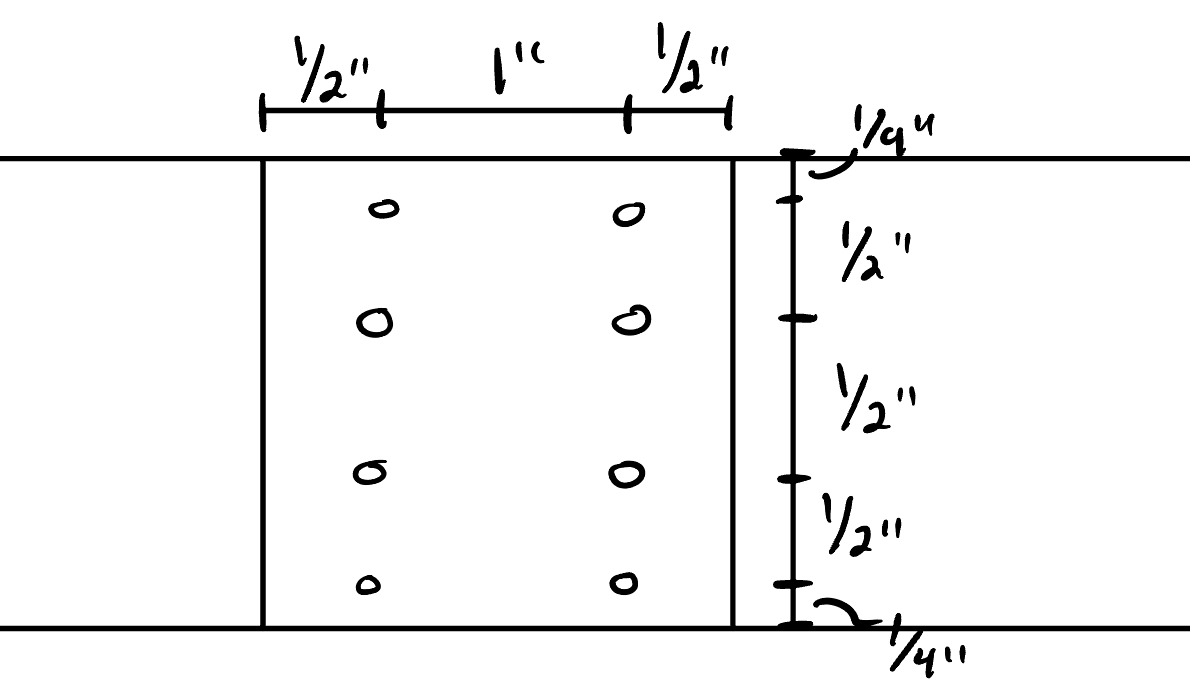
\includegraphics[width=6in]{images/my-design}
\caption{The \num{4} by \num{2} design we chose for our rivet design.}
\label{fig:my-design}
\end{figure}

\begin{align*}
\eta_s&=\num{1.309} \\
\eta_b&=\num{0.9259} \\
\eta_{to}&=\num{1.333} \\
\eta_{t1}&=\num{0.75} \\
\eta_{t2}&=\num{1.5}
\end{align*}

\begin{align*}
F_s&=\qty{1767}{lb} \\
F_b&=\qty{1250}{lb} \\
F_{to}&=\qty{1800}{lb} \\
F_{t1}&=\qty{1012}{lb} \\
F_{t2}&=\qty{506.2}{lb} \\
\sigma_{t1}&=\qty{27}{ksi} \\
\sigma_{t2}&=\qty{13.5}{ksi}
\end{align*}

Given these efficiency factors and forces, we predicted our sample would fail at \qty{1012}{lb} due to the tensile stress in the first row.

\section{Work Assignments} \label{work_assignments}
Refer to Table \ref{table:work_assignments} for the distribution of work during this lab.

\begin{table}[!htbp]
\caption{Work assignments for AER E 322 Lab 3.}
\begin{center}
	\begin{tabular}{| c | c | c | c |}
		\hline
		\multicolumn{1}{| c |}{\textbf{Task}} & \textbf{Matthew} & \textbf{Peter} & \textbf{Natsuki} \\
		\hline
		\multicolumn{4}{| c |}{\textit{Lab Work}} \\
		\hline
		Date Recording & X & X & X \\
		\hline
		Exp. Setup & X & X & X \\
		\hline
		Exp. Work & X & X & X \\
		\hline
		Exp. Clean-Up & X & X & X \\
		\hline
		\multicolumn{4}{| c |}{\textit{Post Lab}} \\
		\hline
		Data Analysis & X & X & \\
		\hline
		\multicolumn{4}{| c |}{\textit{Report}} \\
		\hline
		Introduction & & X & \\
		\hline
		Objectives & & & X \\
		\hline
		Hypothesis & X & & \\
		\hline
		Materials & & & X \\
		\hline
		Apparatus & X & & \\
		\hline
		Procedures & & & X \\
		\hline
		Data & X & X & X \\
		\hline
		Analysis & X & X & X \\
		\hline
		Conclusion & & X & \\
		\hline
		Editing & X & & \\
		\hline
	\end{tabular}
\end{center}
\label{table:work_assignments}
\end{table}

\section{Materials} \label{materials}
\begin{itemize}
\item Two \qty{2}{''} by \qty{8}{''} aluminum sheets \qty{0.025}{''} thick.
\item Rivets with a \qty{0.125}{''} diameter and \qty{0.25}{''} length.
\item Measuring device
\item Clamps
\item Clekos
\item Hole punch
\item Rivet gun
\item Instron machine
\end{itemize}

\section{Apparatus} \label{apparatus}
The Instron tensile machine and the riveted aluminum sample are shown in Figures \ref{fig:instron} and \ref{fig:completed-sample} respectively.

\begin{figure}[htbp]
\centering
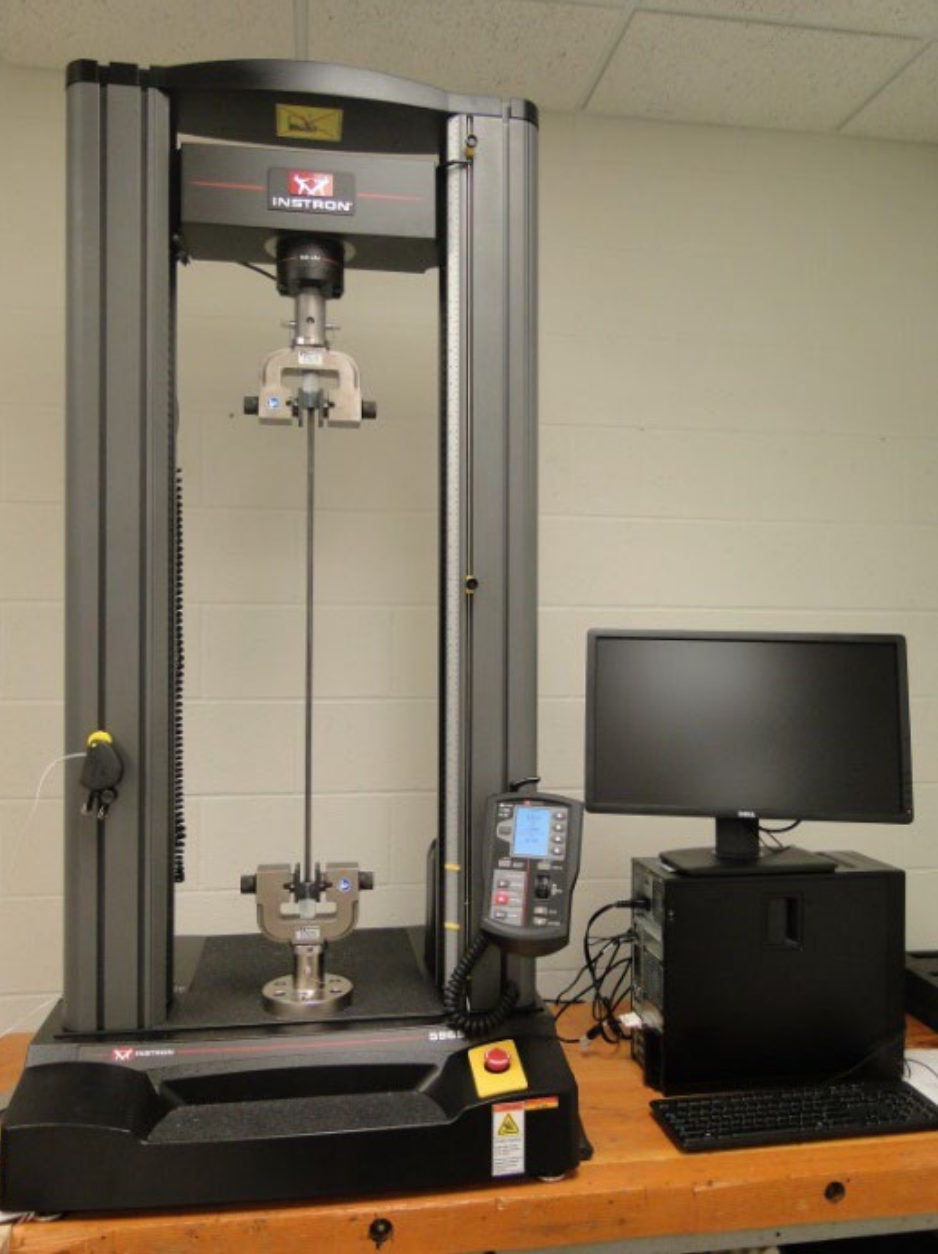
\includegraphics[width=3in]{images/instron}
\caption{The Instron tensile tester.}
\label{fig:instron}
\end{figure}

\begin{figure}[htbp]
\centering
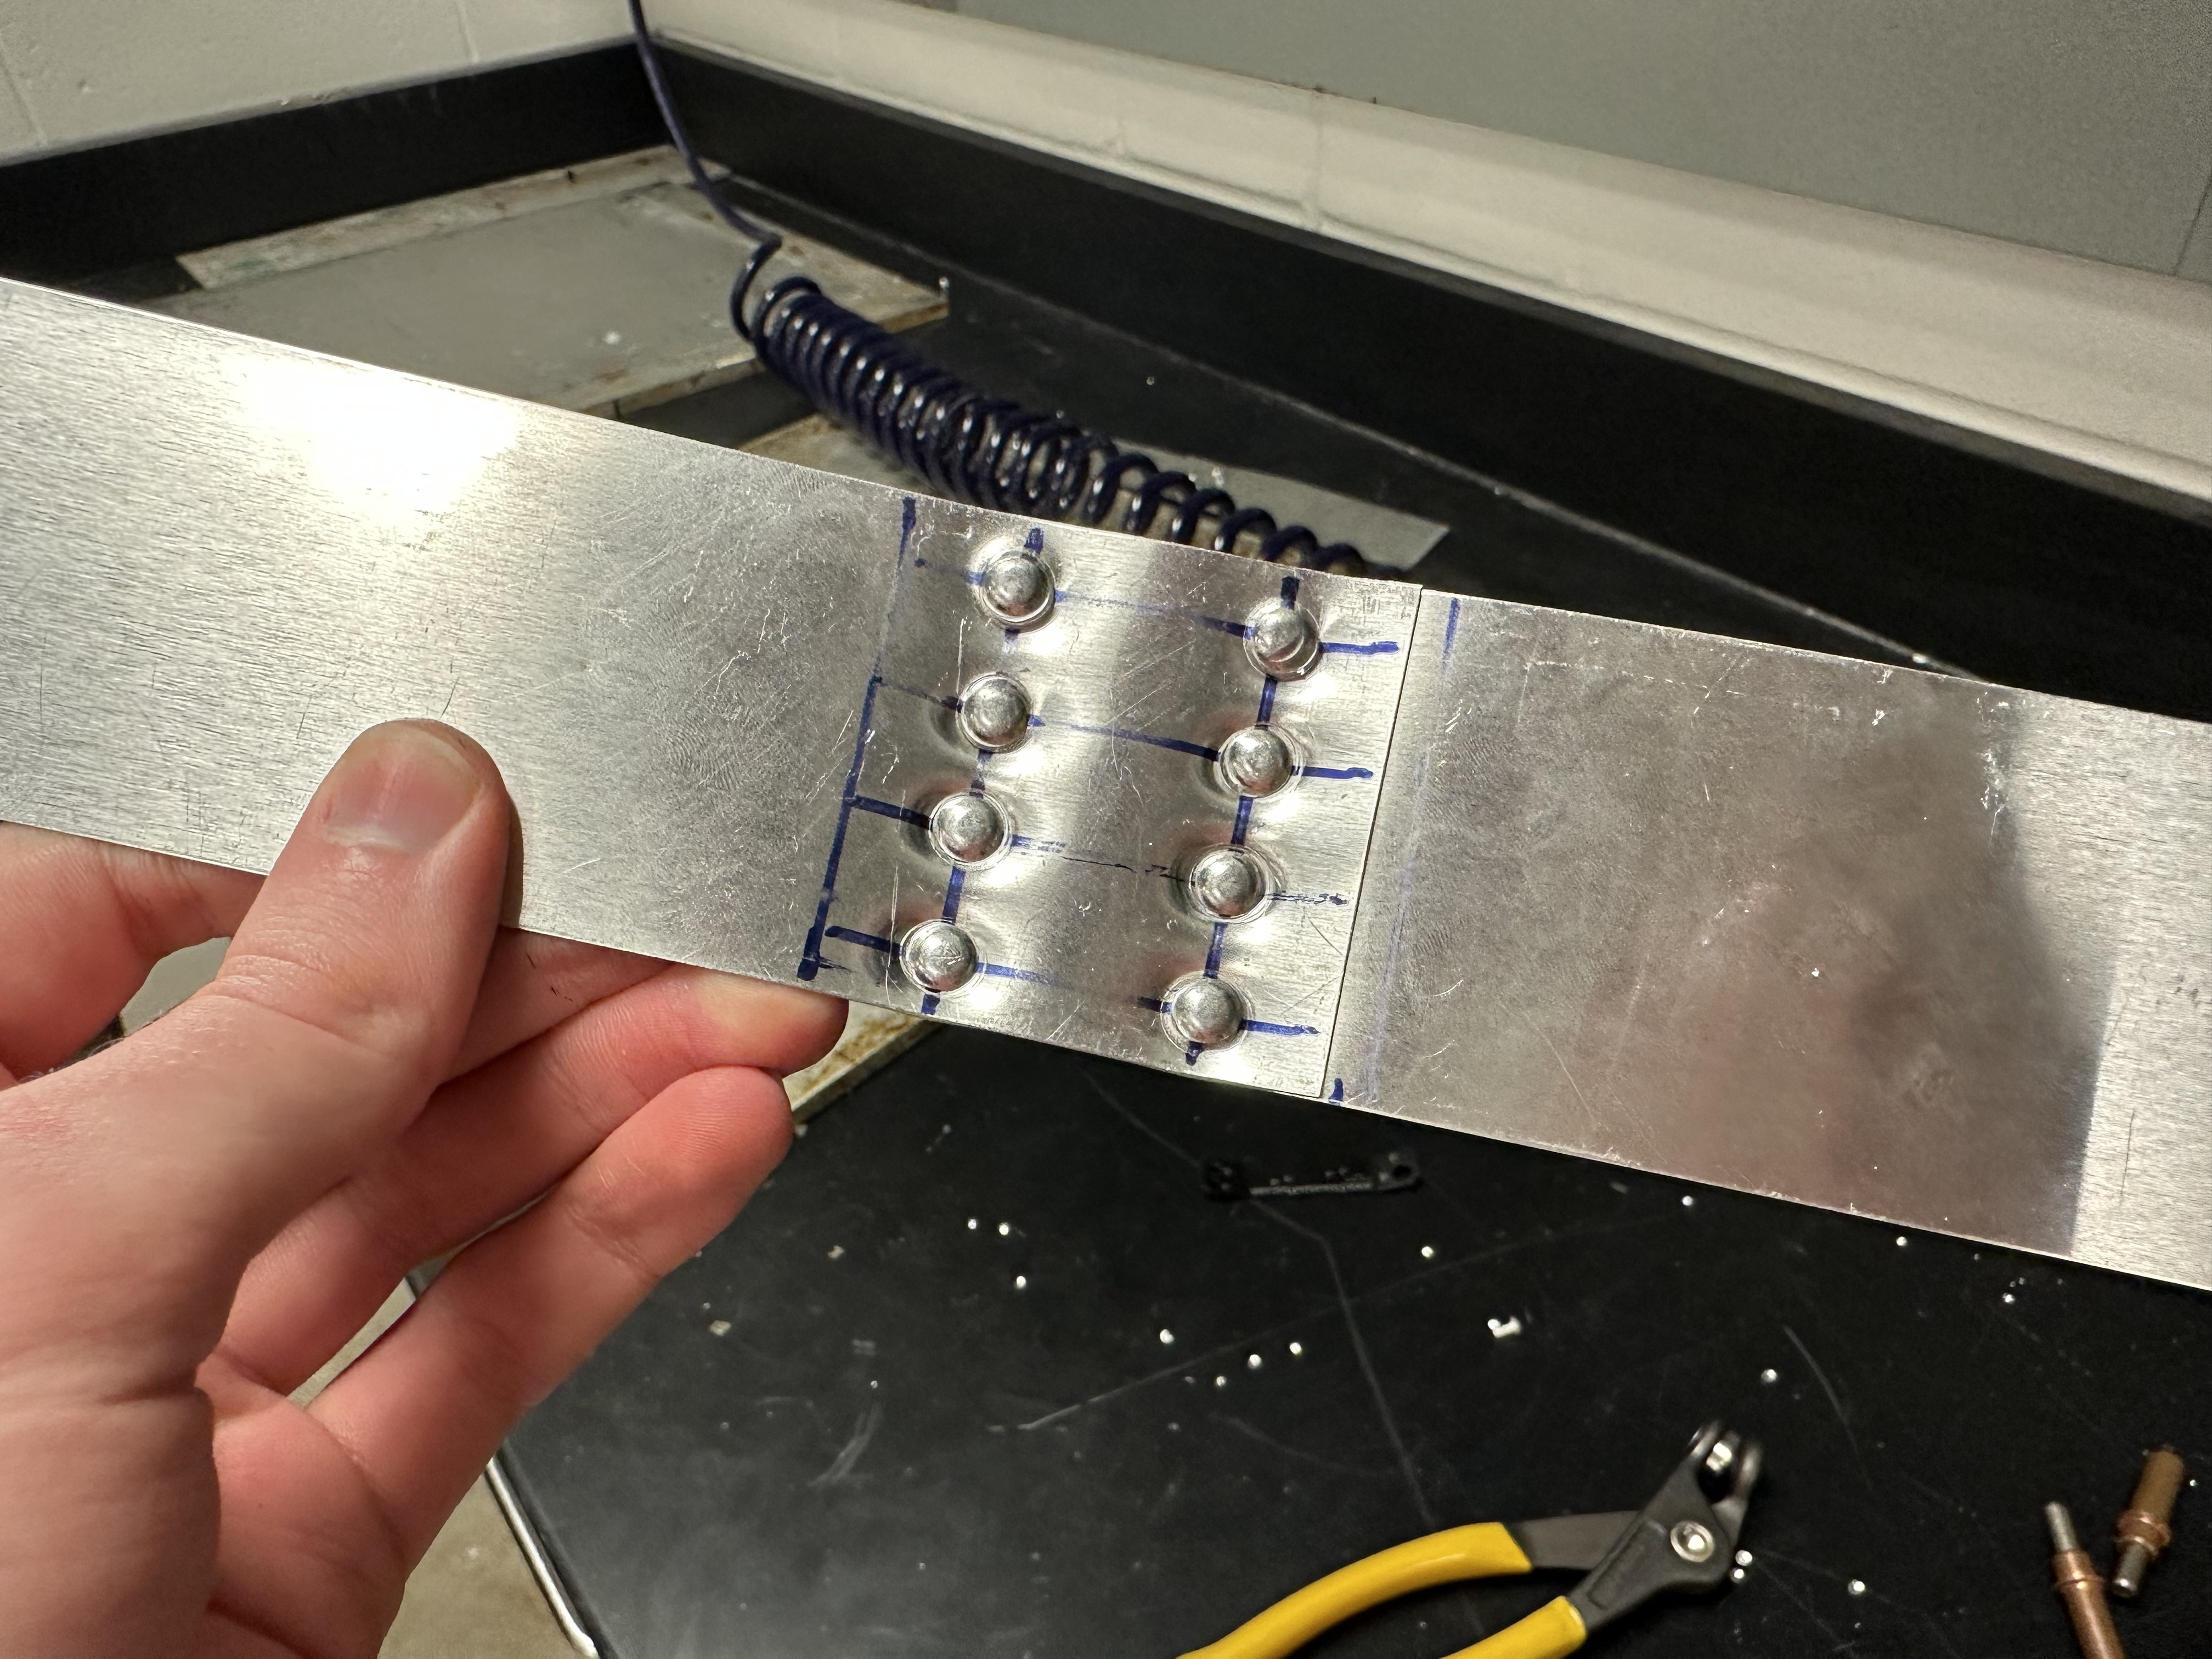
\includegraphics[width=3in]{images/completed-sample}
\caption{The completed sample fully riveted.}
\label{fig:completed-sample}
\end{figure}

\section{Procedures} \label{procedures}
Prepare the two aluminum sheets. Measure a \qty{2}{''} by \qty{2}{''} overlapping area on each aluminum sheet and mark the points on the sample where it will be riveted according to your design. Use the clamps to secure the samples together and punch holes at the appropriate markings---punching both sheets at the same time.

Use the clekos to keep the samples together during riveting but be sure they are not being pressed against the riveting surface or in the way of the riveting gun. Insert a rivet into a hole, place the sample so that the rivet is on the corner of the riveting surface, and then use the riveting gun until the rivet meets your required specifications.

Once the sample is riveted together, place the specimen into the flat-end grips of the Instron. Confirm the distance between the top and bottom is the same. Tighten the grips firmly to the sample, ensuring the sample is taut. See Figure \ref{fig:loaded-sample} for an example.

\begin{figure}[htbp]
\centering
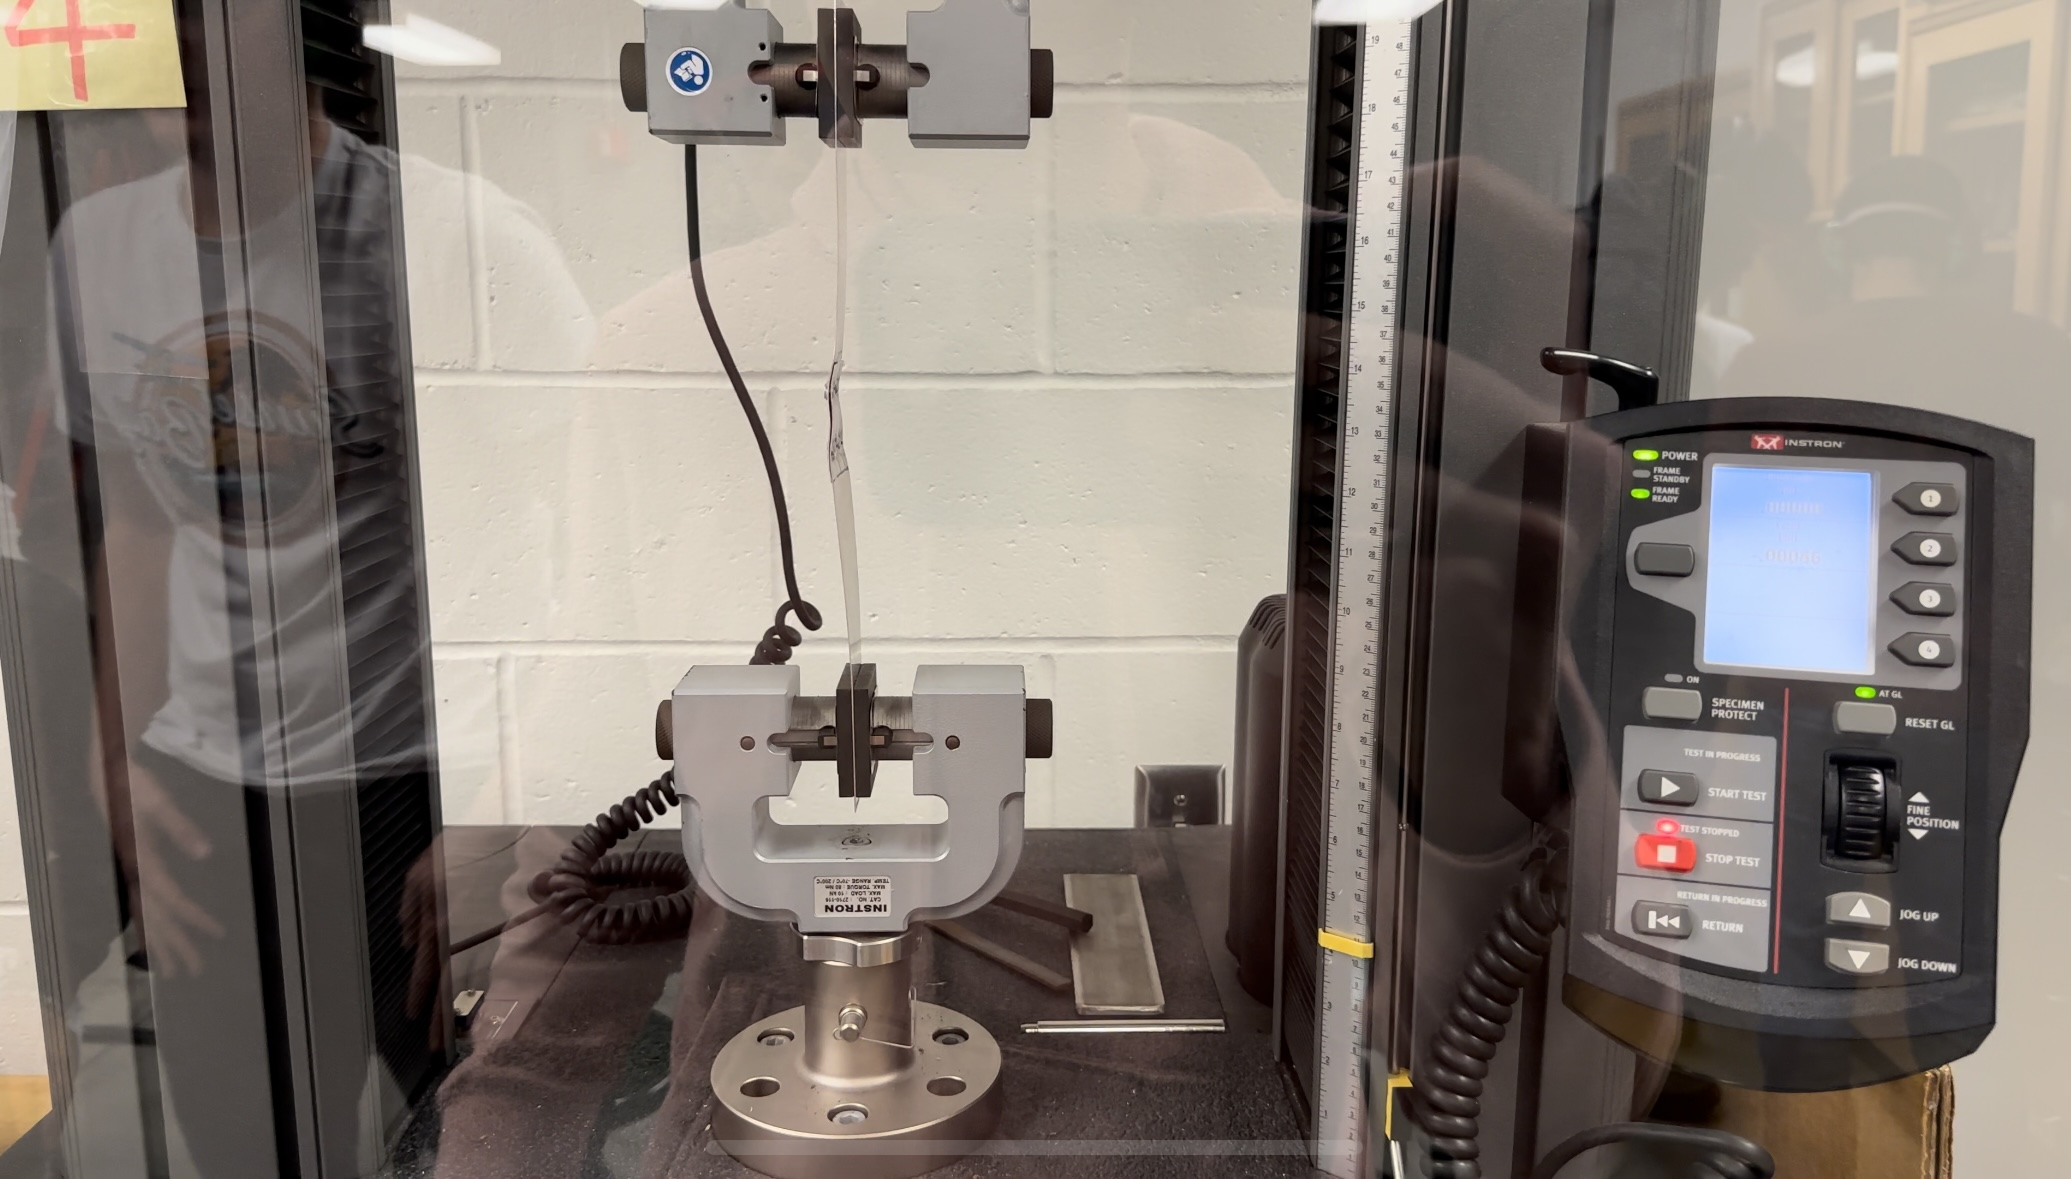
\includegraphics[width=4in]{images/loaded-sample}
\caption{The riveted aluminum sample loaded into the Instron machine.}
\label{fig:loaded-sample}
\end{figure}

Press ``Balance All'' in the Bluehill 3 software. In the software, create a new file and set the stress to increase at \qty{10}{lb/\s}. For safety, stand at least \qty{2}{ft} away from the Instron with a safety glass between you and the machine. Start the tensile test and run it until the sample fails. Recover the sample from the Instron, save the test data, and take pictures of the failed sample.

\section{Data} \label{data}
As shown in the Stress-Strain curve, Figure \ref{fig:stress-strain}, our sample endured a maximum stress of \qty{17.66}{ksi}, a maximum strain of \qty{0.0203}{in/in}, and a maximum force of \qty{882.9}{lb}.

\begin{figure}[htbp]
\centering
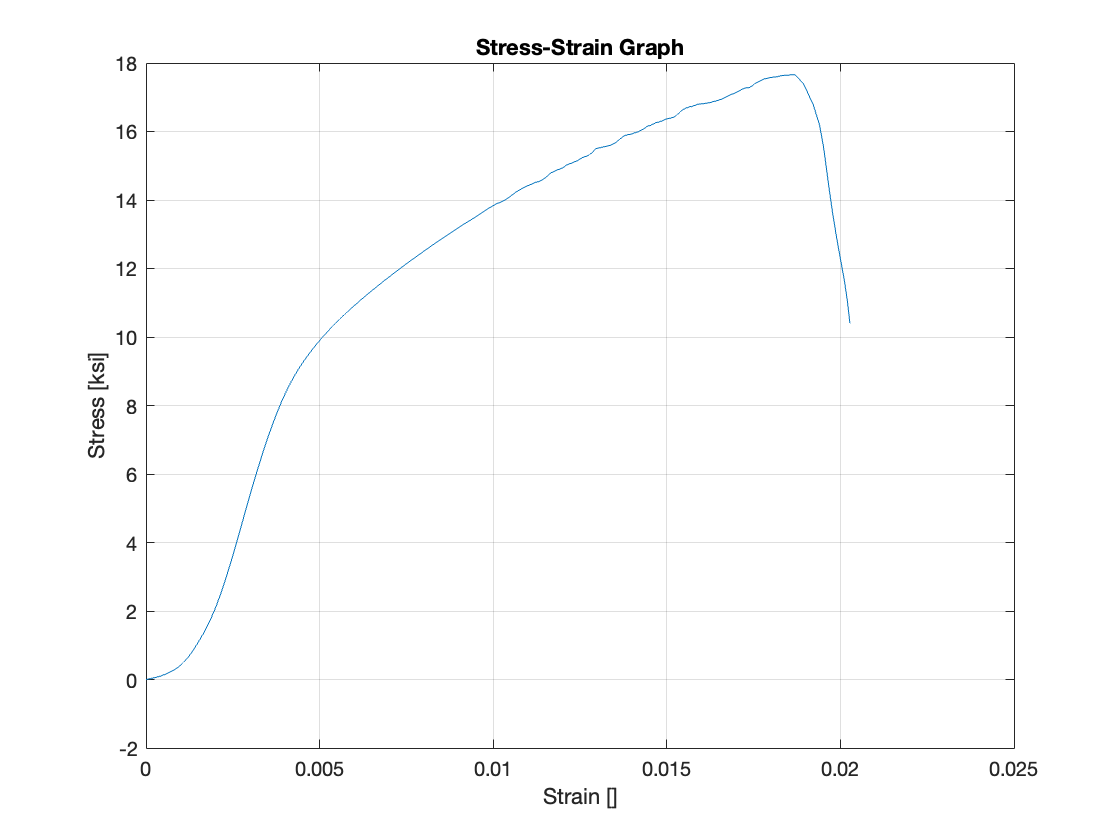
\includegraphics[width=4in]{images/Graphs/stress-strain}
\caption{The stress-strain curve of our sample while undergoing a tensile stress test in the Instron machine.}
\label{fig:stress-strain}
\end{figure}

\section{Analysis} \label{analysis}
Two of our group members chose a 1-3-1 design and the other group member chose a 4-4 design. We used the 4-4 design because it had the highest minimum load required for failure. The lowest joint efficiency factor for the 1-3-1 design was $\eta_b$, the bearing joint efficiency factor, which we calculated to be \num{0.5787}. Based on this efficiency, the minimum force required for failure was \qty{781.3}{lb}---resulting in bearing failure. The lowest joint efficiency factor for the 4-4 design was $\eta_{t1}$, the tensile joint efficiency of the first row, which was calculated to be \num{0.75}. Based on this efficiency, the minimum force required for failure was \qty{1012}{lb}. Since the 4-4 design had the higher minimum force required for failure, we chose the 4-4 design for our lab.

As shown in Figure \ref{fig:failed-sample}, our sample failed due to tensile stress in the first row.

\begin{figure}[htbp]
\centering
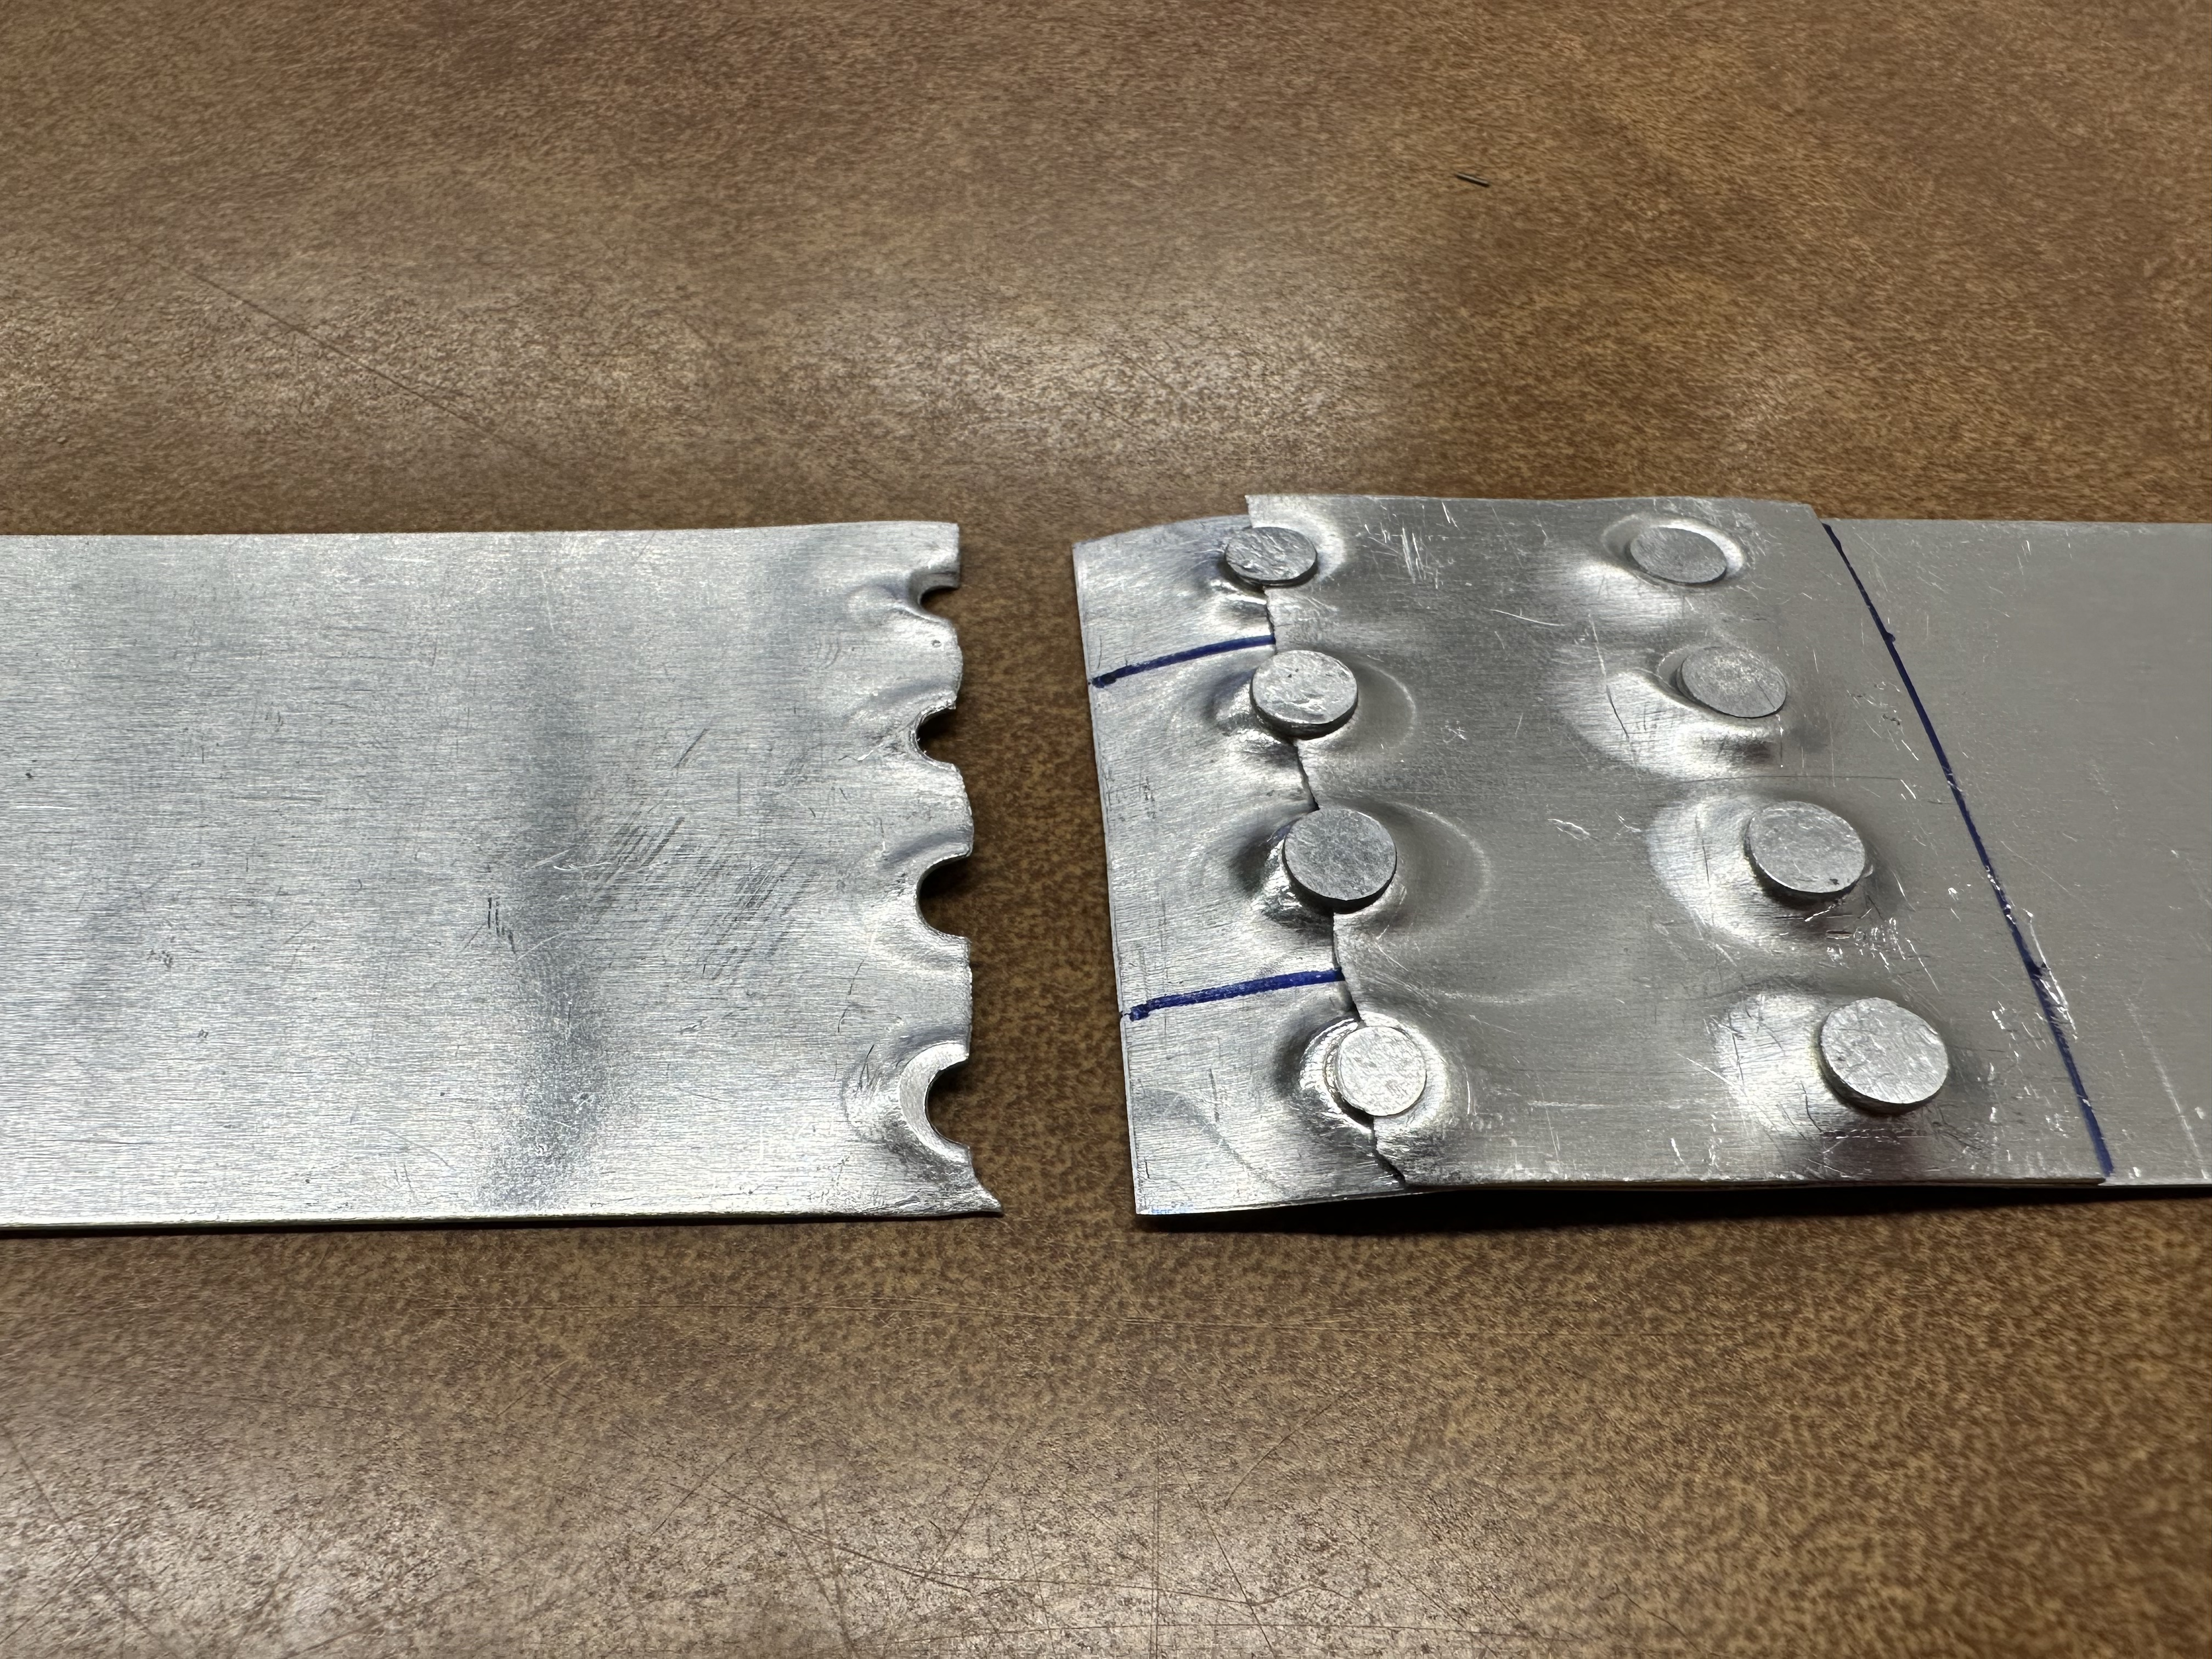
\includegraphics[width=4in]{images/failed-sample}
\caption{A close-up of the failed sample, showing the first row tensile stress failure.}
\label{fig:failed-sample}
\end{figure}

This matches our hypothesis and calculations, however, the failure occurred prematurely according to our calculations. In general, we argue that the sampled failed due to tensile stress because we lacked a third row to distribute the tensile stress. Since we only had two rows, most of the stresses were concentrated in the first row.

Another design reason for the premature failure, however, was the amount of space between each rivet. According to the definition of stress, as the area increases, stress decreases. Since we minimized the area between the rivets, the tensile stress forces were maximized within the rows.

According to the MIL-R-47196A specifications, the driven head diameter should be a minimum of \qty{0.163}{in} and ours were roughly \qty{0.245}{in}. Although the driven head diameter surpassed the specifications, our driven head thickness did not: according to MIL-R-47196A, the driven head thickness should be \qtyrange{0.05}{0.07}{in}, and our driven head thickness averaged \qty{0.037}{in}. Additionally, the four rivets closest to the long edges of the sample were all riveted at a slight angle as opposed to perpendicular. Lastly, after hole punching and riveting, the sample was slightly bowed, especially on the edges. These manufacturing issues could have been a factor that led to the premature failure.

One of the most significant causes of premature failure, however, was a manufacturing defect in the first row. If you closely observe the bottom-leftmost rivet in Figure \ref{fig:failed-sample}, you will note that the rivet appears visually smaller than the others. This rivet had a driven head thickness of \qty{0.001}{in}---significantly lower than the specifications required---and it was driven at an angle. Observing the side of the failed sample without the rivets, you will note the extreme plastic deformation that occurred around the poorly manufactured rivet. It is highly likely that this under-specced rivet created a stress concentrator near the edge of the sample which caused the sample to fail locally, and then propagate the failure across the entire row.

Despite the manufacturing defects, our sample was designed and manufactured to meet the design guidelines provided in the lecture notes. 

\section{Conclusion} \label{conclusion-section}
We accurately predicted the type of failure our rivet design would undergo, however, due to manufacturing inconsistencies, our design failed prematurely according to our calculations. This highlights the importance of building factors of safety and proper quality control procedures into our engineering designs. It only takes one bad component to cause catastrophic failure.

\end{document}
